\section{Preliminaries}\label{sc:background}
This section describes the preliminaries to understand the work described in the paper.

\subsection{Maude /Rewriting Logic}
\simon{Peter, I guess you have some text for this section.}

\subsubsection{Model checking}
\simon{Is this section needed?}


\subsection{Co-simulation}
Co-simulation enables global simulation of a system consisting of multiple black-box SUs. 
An SU has a dedicated solver calculating the behaviour trace of the dynamical system it represents. 
A dynamical system represents a function from time and space into some often multi-dimensional and continuous space. 
Examples include population growth, water flow, and pendulums. 
Interaction of the system with the external environment happens through inputs and outputs~\cite{Gomes2019a,Kubler2000}.

SUs are coupled through their inputs and outputs.
A coupling indicates that the state of one SU is reliant on the state of another SU.
A coupling can be seen as an invariant saying that the value on a coupled input and output must be identical at all times - known as a coupling restriction. 
However, in practice, the coupling restrictions can only be satisfied at specific points in time, referred to as communication points. 
Therefore, each SU makes assumptions about the evolution of the input values between the communication points to satisfy the invariant.
These assumptions cause accumulable errors in the co-simulation~\cite{Arnold2014}.

The orchestrator computes the behavioural trace of all SUs and tries to satisfy their coupling restrictions by exchanging values. 
The orchestrator aims to find the communication points minimizing the co-simulation error while ensuring that the SUs move in lockstep. 
Studies \cite{Gomes2019,Oakes2021,Gomes2018f,Schweizer2015c,Gomes2018a} show that optimal communication points depend on the implementation of the SUs.

We now introduce our definition of an SU in \cref{def:fmu}.
The definition is based on \cite{Broman2013,Gomes2019c,thrane2021} and represents an abstract version of an SU.

\begin{definition}[Simulation Unit]\label{def:fmu}
  An SU with identifier $c$ is represented by the tuple
  $$\tuple{\stateset{c}, \inputs{c}, \outputs{c}, \fset{c}, \fget{c}, \fdoStep{c}},$$
  where:
  \begin{compactitem}
    \item $\stateset{c}$ represents the state space.
    \item $\inputs{c}$ and $\outputs{c}$ the set of input and output variables, respectively.
    The union of the inputs and outputs is called the variables of the SU:
    $\variables{c} = \inputs{c} \cup \outputs{c}$ 
    \item $\values$ is the set of values that a variable can hold and let $\valuesExchanged: \timebase \times \values$ be the set of abstract values exchanged between input and output variables.
    The functions
    $\fset{c} : \stateset{c} \times \inputs{c} \times \valuesExchanged \to \stateset{c}$ and $\fget{c}: \stateset{c} \times \outputs{c} \to \valuesExchanged$ respectively sets an inputs and gets an outputs. 
    \item $\fdoStep{c}: \stateset{c} \times \stepbase \to \stateset{c} \times \stepbase $ is a function that instructs the SU to compute its state after a given time duration. If an SU is in state $\stateafter{c}{t}$ at time $t$, $(\stateafter{c}{t+h}, h) = \fdoStep{c}(\stateafter{c}{t}, H)$ approximates the state $\stateafter{c}{t+h}$ of the corresponding model at time $t+h$, where $h \leq H$. 
  \end{compactitem}
\end{definition}

The state of SU $A$ at time $t$ is denoted $\stateafter{A}{t}$.
The function $\fdoStep{c}$ returns a step size because some SUs implement error estimation and may conclude that taking a step size of $H$ will result in an intolerable error meaning the SU takes a smaller step than planned.

A collection of coupled SUs forms a scenario.
We provide a formal description of a scenario in \cref{def:cosim_scenario}.

\begin{definition}[Scenario]\label{def:cosim_scenario}
  A scenario is a structure $\tuple{\fmus, \coupling, \mayReject, \allfeedthroughs, \allreactivity, \alldelayed}$ where 
  \begin{compactitem}
    \item Each identifier $c \in \fmus$ is associated with an SU, as defined in \cref{def:fmu}
    \item $\coupling(u)=y$ means that the output $y$ is connected to input $u$.   
    Let $\allinputs = \bigcup_{c \in \fmus} \inputs{c}$ and $\alloutputs = \bigcup_{c \in \fmus} \outputs{c}$, then $\coupling : \allinputs \to \alloutputs$. 
    \item $\mayReject \subseteq \fmus$ denotes the SUs that implement error estimation. 
    \item The function
    $\allreactivity : \allinputs \to \mathbb{B}$ is total and provide non-confidential information about the SUs' input approximation functions.
    $\allreactivity(\inputvar{c}) = \true$ means that the function $\fdoStep{c}$ assumes that the timestamp $t_{SU}$ of the state of SU $c$ ($\stateafter{c}{t_{SU}}$) is less than the timestamp $t_v$ of the value $v = \tuple{t_V,\dontcare}$ set on the input $\inputvar{c}$.
    \item  Finally, the set of feed-through components, $\allfeedthroughs = \bigcup_{c \in \fmus} \feedthrough{c}$, where the input $\inputvar{c} \in \inputs{c}$ feeds through to output $\outputvar{c} \in \outputs{c}$, that is, $(\inputvar{c},\outputvar{c}) \in \feedthrough{c}$, when there exists $v_1, v_2 \in \valuesExchanged$ and $\state{c} \in \stateset{c}$, such that
    $\fget{c} (\fset{c}(\state{c}, \inputvar{c}, v_1), \outputvar{c}) \neq \fget{c} (\fset{c}(\state{c}, \inputvar{c}, v_2), \outputvar{c}).$
  \end{compactitem}
\end{definition}

We have based \cref{def:cosim_scenario} on the FMI standard. 
However, feed-through and reactivity are extensions of the standard, introduced to cover a broad class of co-simulation scenarios.
We use the syntax in \cref{fig:simpleexample} to graphically present co-simulation scenarios.

\begin{figure}[htb]
  \centering
  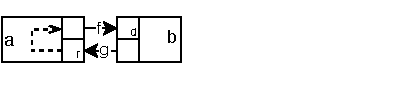
\includegraphics[width=0.7\textwidth]{images/simple_example.pdf}
  \caption{A co-simulation scenario ($S1$).}
  \label{fig:simpleexample}  
\end{figure}

\subsubsection{Instrumentation}
We refer to an input variable $\inputvar{c} \in \allinputs \land \neg \allreactivity(\inputvar{c})$ as a delayed input. 
While an input variable $\inputvar{c}$ where $\inputvar{c} \in \allinputs \land \allreactivity(\inputvar{c})$ is referred to as a reactive input. 

The function $\allreactivity$ is the instrumentation of the scenario.
The instrumentation describes the input approximation functions of the different SUs.
%An example of the instrumentation function
Changing the instrumentation of a scenario changes the algorithm used to simulate the scenario.
We assume that the instrumentation of a scenario is constant through the simulation, which is the case for most commercially used SUs.

\subsection{Co-simulation algorithms}\label{sc:cosimalgo}
The orchestrator simulates the scenario by interpreting/executing a co-simulation algorithm on the scenario.

A co-simulation algorithm consists of an initialization procedure, a co-simulation step, and some additional FMI functions changing the mode of an SU~\cite{FMI2014}.
Our work concentrates in the paper on the co-simulation step, which we refer to as the algorithm throughout the paper. 
The reason is that the other aspects of a co-simulation algorithm can be derived from the presented method.  

The algorithm changes the co-simulation state. 
Our work is performed using an abstract co-simulation state, which is defined as the combination of the state of the individual SUs in \cref{def:cosimstate}.

\Cref{def:runtime_state} defines the abstract state of an SU.

\begin{definition}[Abstract State]\label{def:runtime_state}
  Given an SU $c$ as defined in \cref{def:fmu}, the observable abstract state of $c$ is a member of the set $\runstate{c} = \timebase \times \runstate{\inputs{c}} \times \runstate{\outputs{c}} \times \runstate{V_c}$, where:
  \begin{compactitem}
    \item $\timebase$ is the time of the SU meaning the state of the SU is $\stateafter{c}{t}$,
    \item $\runstate{\inputs{c}} : \inputs{c} \to \timebase$ is a total function linking each input port with its timestamp.  
    \item $\runstate{\outputs{c}} : \outputs{c} \to \timebase$ is a total function linking each output port with its timestamp.  
    \item $\runstate{V_c} : \variables{c} \to \values$ is a total function linking each port with a its value.  
  \end{compactitem}
\end{definition}

We use the abstract state $\runstate{c}$ of an SU $c$ instead of the internal state $\stateset{c}$ defined in \cref{def:fmu} because the orchestrator cannot observe the later.

\begin{definition}[Abstract Co-simulation State]\label{def:cosimstate}
  Given a co-simulation scenario $\tuple{\fmus, \coupling}$, as defined in \cref{def:cosim_scenario}, the abstract co-simulation state is a member of the set $\runstate{\fmus} = \prod_{c \in \fmus} \runstate{c}$. 
\end{definition}

A co-simulation step $P$ is a sequence of the functions $\fset{c},\fget{c}$, and $\fdoStep{c}$ described in \cref{def:fmu}.
It simulates the scenario by advancing all SUs $\fmus$ from an initial state at time $t$ to a final state at time $t+H, \textrm{ where } H > 0$.
The co-simulation must ensure that the coupling restrictions are satisfied at both the initial and final state.

\Cref{fig:algorithms} shows three different co-simulation steps of the scenario in \cref{fig:simpleexample}.
The three different algorithms are all allowed by the FMI standard~\cite{FMI2014}. 

\begin{figure}[htb]
  \centering
  \begin{minipage}[t]{.325\textwidth}
    \begin{algorithm}[H]
      \caption{}
      \label{alg:algorithm_1}
      \begin{algorithmic}[1]
        \scriptsize
        \State $(\stateafter{A}{H},H) \gets \fdoStep{A}(\stateafter{A}{0}, H)$
        \State $(\stateafter{B}{H},H) \gets \fdoStep{B}(\stateafter{B}{0}, H)$
        \State $f_{v} \gets \fget{A}(\stateafter{A}{H}, \outputvar{f})$
        \State $g_{v} \gets \fget{B}(\stateafter{B}{H}, \outputvar{g})$
        \State $\stateafter{B}{H} \gets \fset{B}(\stateafter{B}{s}, \inputvar{f}, f_{v})$
        \State $\stateafter{A}{H} \gets \fset{A}(\stateafter{A}{H},\inputvar{g},g_{v})$
      \end{algorithmic}
    \end{algorithm}
  \end{minipage}
  \begin{minipage}[t]{0.325\textwidth}
    \begin{algorithm}[H]
      \caption{}
      \label{alg:algorithm_2}
      \begin{algorithmic}[1]
        \scriptsize
        \State $(\stateafter{B}{H},H) \gets \fdoStep{B}(\stateafter{B}{0}, H)$
        \State $(\stateafter{A}{H},H) \gets \fdoStep{A}(\stateafter{A}{0}, H)$
        \State $g_v \gets \fget{B}(\stateafter{B}{H}, \outputvar{g})$
        \State $\stateafter{A}{H} \gets \fset{A}(\stateafter{A}{H}, \inputvar{g}, g_v)$
        \State $f_v \gets \fget{A}(\stateafter{A}{H}, \outputvar{f})$
        \State $\stateafter{B}{H} \gets \fset{B}(\stateafter{B}{H}, \inputvar{f}, f_v)$
      \end{algorithmic}
    \end{algorithm}
  \end{minipage}
  \begin{minipage}[t]{0.325\textwidth}
    \begin{algorithm}[H]
      \caption{}
      \label{alg:algorithm_3}
      \begin{algorithmic}[1]
        \scriptsize
        \State $(\stateafter{B}{H},H) \gets \fdoStep{B}(\stateafter{B}{0}, H)$
        \State $g_v \gets \fget{B}(\stateafter{B}{H}, \outputvar{g})$
        \State $\stateafter{A}{0} \gets \fset{A}(\stateafter{A}{0}, \inputvar{g}, g_v)$
        \State $f_v \gets \fget{A}(\stateafter{A}{0}, \outputvar{f})$
        \State $\stateafter{B}{H} \gets \fset{B}(\stateafter{B}{H}, \inputvar{f}, f_v)$
        \State $(\stateafter{A}{H},H) \gets \fdoStep{A}(\stateafter{A}{0}, H)$
      \end{algorithmic}
    \end{algorithm}
    \vspace{4pt}
  \end{minipage}
  \vspace{-2em}
  \caption{Three algorithms conforming to the FMI Standard (version 2.0) of the scenario in \cref{fig:simpleexample}.}
  \label{fig:algorithms}
\end{figure}

Although the three algorithms in \cref{fig:algorithms} consist of the same actions, they are not equivalent, and simulating with one algorithm instead of one of the others could drastically change the co-simulation result as shown in \cite{Gomes2019c,hansen_verification_2021}. 
At the end of \cref{sec:correctcosim}, we show which of these algorithms is correct.

The purpose of the co-simulation step $P$ is defined in \cref{def:comsim_step}.

\begin{definition}[Co-simulation Step]\label{def:comsim_step}
  A co-simulation step $P$ is correct starting from the abstract state $\runstate{}$ if:
  \begin{align}
    &\fpreCoSimStep(\tuple{t,\runstate{\allinputs}, \runstate{\alloutputs},\runstate{V}}, t) \triangleq 
    \forall \inputvar{c} \in \allinputs
    \exists \outputvar{d} \in \alloutputs
    \cdot \coupling(\inputvar{c}) = \outputvar{d}  \nonumber \\
    &\qquad \qquad \qquad \qquad \qquad \implies
    \runstate{V}(\inputvar{c}) = \runstate{V}(\outputvar{d}) \nonumber \\
    &[\fpreCoSimStep(\runstate{}, t), 
    \fpreCoSimStep(\after{\runstate{}}, t+H)] 
    \langle \after{\runstate{}} \gets P\rangle
  \end{align}
\end{definition}

$\runstate{} = \tuple{t, \runstate{\allinputs}, \runstate{\alloutputs}, \runstate{V}}$ means that all SUs are at time $t$ and $\runstate{\allinputs} = \prod_{c \in \fmus}\runstate{\inputs{c}}$ and $\runstate{\alloutputs} = \prod_{c \in \fmus}\runstate{\outputs{c}}$.
\Cref{def:comsim_step} shows that the precondition and postcondition of the co-simulation step are the same ($\fpreCoSimStep$).
It says that all SUs are synchronized and that all the coupling restrictions are satisfied.

The three Algorithms in \cref{fig:algorithms} all satisfy the criteria of \label{eq:co_sim_step} even though they can result in utterly different simulation results.
To discriminate between them, we need to look into the semantics of the different actions from \cref{def:fmu}, which we describe next in \cref{def:getout,def:setin,def:step}.

We base our semantic on \cite{Gomes2019a,hansen_verification_2021}.
\simon{Make reference to }
Due to space limitations we limitations we refer readers to these papers for a deeper explanation of the actions.

\begin{definition}[Get Action]\label{def:getout}  
  For an SU $c$ at timestamp $t$ with the abstract state $\runstate{c} = \tuple{t,\runstate{\inputs{c}}, \runstate{\outputs{c}}, \runstate{V_c}}$ the effect of obtaining a value from an output $\outputvar{c}$ using the action $\fget{c}(\stateafter{c}{t},\outputvar{c})$ is described using the specification statement:
  \begin{align}
    &\fpreget{c}(\outputvar{c}, \tuple{t,\runstate{\inputs{c}}, \runstate{\outputs{c}}, \runstate{V_c}}) \triangleq
    \runstate{\outputs{c}}(\outputvar{c}) < t \land \nonumber \\
    & \qquad \qquad \qquad \qquad \qquad 
    \forall \inputvar{c} \in \inputs{c} \cdot (\inputvar{c}, \outputvar{c}) \in \feedthrough{c} 
    \implies \runstate{\inputs{c}}(\inputvar{c}) = t  \nonumber \\
    &\fpostget{c}(\outputvar{c}, \tuple{t,\runstate{\inputs{c}}, \runstate{\outputs{c}}}, \tuple{t,\runstate{\inputs{c}}, \after{\runstate{\outputs{c}}}}, v) \triangleq 
    \after{\runstate{\outputs{c}}}(\outputvar{c}) = t \nonumber \\
    & \qquad \qquad \qquad \qquad \qquad 
    \land 
    \forall \outputvar{m} \in (\outputs{c} \setminus \outputvar{c}) \cdot 
    \after{\runstate{\outputs{c}}}(\outputvar{m}) =
    \runstate{\outputs{c}}(\outputvar{m})\nonumber\\
    &\qquad \qquad \qquad \qquad \qquad \land
    \after{\runstate{V_c}}(\outputvar{c})= v \nonumber\\
    &[\fpreget{c}(\outputvar{c}, \runstate{c}), 
    \fpostget{c}(\outputvar{c}, \runstate{c}, \after{\runstate{c}}, v)] 
    \langle (v, \after{\runstate{c}}) \gets \fget{c}(\stateafter{c}{t},\outputvar{c}) \rangle \nonumber
  \end{align}
\end{definition}

\begin{definition}[Set Action]\label{def:setin}
  For an SU $c$ at timestamp $t$ with the abstract state $\runstate{c} = \tuple{t,\runstate{\inputs{c}}, \runstate{\outputs{c}}, \runstate{V_c}}$ the effect of 
  setting a value $\inputV = \tuple{t_{V}, X}$ on the input $\inputvar{c}$ using the action $\fset{c}(\stateafter{c}{t}, \inputvar{c}, \inputV)$ is described using the specification statement:
    \begin{align}
      &\fpreset{c}(\inputvar{c}, \tuple{t_{V},X}, \tuple{t,\runstate{\inputs{c}}, \runstate{\outputs{c}}, \runstate{V_c}}) \triangleq 
      let\; t_s = \runstate{\inputs{c}}(\inputvar{c}) \; in \; t_s < t_{V} \nonumber \\
      & \qquad \qquad \qquad \qquad \qquad
      \land 
      ((\reactivity{c}(\inputvar{c}) \land t_s = t) 
      \lor (\neg\reactivity{c}(\inputvar{c}) \land t_s < t)) \nonumber \\
      &\fpostset{c}(\inputvar{c}, \tuple{t_{V},X}, \tuple{t,\runstate{\inputs{c}}, \runstate{\outputs{c}}, \runstate{V_c}}, 
      \tuple{t, \after{\runstate{\inputs{c}}} \runstate{\outputs{c}}, \after{\runstate{V_c}}}) \triangleq 
      t_{V} = \after{\runstate{\inputs{c}}}(\inputvar{c})
      \nonumber\\
      &\qquad \qquad \qquad \qquad \qquad \land
      \forall \inputvar{m} \in (\inputs{c} \setminus \inputvar{c}) \cdot 
      \after{\runstate{\inputs{c}}}(\inputvar{m}) =
      \runstate{\inputs{c}}(\inputvar{m}) 
      \nonumber \\
      &\qquad \qquad \qquad \qquad \qquad \land
      \after{\runstate{V_c}}(\inputvar{c}) = X \nonumber\\
      &[\fpreset{c}(\inputvar{c}, \runstate{c}), 
      \fpostset{c}(\inputvar{c}, \inputV, \runstate{c}, \after{\runstate{c}})] 
      \langle \after{\runstate{c}} \gets \fset{c}(\stateafter{c}{t},\inputvar{c}, \inputV) \rangle \nonumber
    \end{align}
  \end{definition}


  \begin{definition}[Step Computation]\label{def:step}
    For an SU $c$ at timestamp $t_{SU}$ with the abstract state $\runstate{c} = \tuple{t_{SU},\runstate{\inputs{c}}, \runstate{\outputs{c}, \runstate{V_c}}}$ the effect of stepping it with the step duration $H$ using the action $\fdoStep{c}(\stateafter{c}{t}, H)$ is defined using the following specification statement:
    \begin{align}
      &\fpredoStep{c}(H, \tuple{t,\runstate{\inputs{c}}, \runstate{\outputs{c}, \runstate{V_c}}}) \triangleq 
      \forall \inputvar{c} \in \inputs{c}
      \cdot 
      ((\reactivity{c}(\inputvar{c}) \land t_{SU} + H = \runstate{\inputs{c}}(\inputvar{c}))
      \nonumber \\
      &\qquad \qquad \qquad \qquad \qquad \qquad \qquad \qquad \qquad 
      \lor 
      (\neg \reactivity{c}(\inputvar{c}) \land t_{SU} = \runstate{\inputs{c}}(\inputvar{c})))
      \nonumber \\
      &\fpostdoStep{c}(H, \tuple{t,\runstate{\inputs{c}}, \runstate{\outputs{c}}, \runstate{V_c}}, \tuple{t',\runstate{\inputs{c}}, \runstate{\outputs{c}}, \after{\runstate{V_c}}}) \triangleq t + H = t' \nonumber \\
      &[\fpredoStep{c}(H, \runstate{c}), 
      \fpostdoStep{c}(H, \runstate{c}, \after{\runstate{c}})] 
      \langle (\after{\runstate{c}}, H) \gets \fdoStep{c}(\stateafter{c}{t},H) \rangle \nonumber
    \end{align}
  \end{definition}

%   \cref{def:step} describes that to advance the state of an SU, all its inputs must have been correctly updated with respect to their contract since the last $\fdoStep{c}$ action. 
%   By updating the inputs, we mean that their inputs have been properly advanced in time by the $\fset{c}$ action defined in \cref{def:setin}.   
%   This is informally what $\fpredoStep{c}$ says.

%   The effect of stepping an SU is that the SU's abstract state gets advanced with the duration $H$ this is defined by $\fpostdoStep{c}$.
%   Note that we, for now, assume that an SU will accept all step duration. 
%   Step rejection is described in \vref{sc:complex}.

%   \cref{def:step,def:setin,def:getout} describe the semantics of the actions, both their precondition and effect on the co-simulation state.



\subsection{Complex Scenarios}
Complex scenarios are subject to algebraic loops or step rejections.
A complex scenario is simulated using an iterative orchestration algorithm.
\simon{Add scenario /figure}

The algorithm is iterative because the orchestrator needs to adapt to the behavior of the SUs to satisfy the constraints associated with each SU, account for possible step rejections, and solve algebraic loops. 
The orchestrator achieves this by finding a correct valuation of all inputs and outputs in the scenario.
The valuation defines the step duration and the values it uses to solve the scenario's algebraic loops. 
A correct valuation ensures that all SUs agree on the step duration and solves all algebraic loops by finding a fixed point.
A co-simulation can only be correctly simulated using a correct valuation.

The orchestrator must find a correct valuation in every co-simulation step because it depends on the current internal state of the SUs, which varies from one co-simulation step to the next.

Due to space limitations, we will not describe the process for finding a correct valuation. 
Interested readers are referred to \cite{thrane2021}.

\subsection{Correct Co-simulation Algorithms}\label{sec:correctcosim}
To optimally simulate a co-simulation scenario using an algorithm $P$ requires more than a correct valuation $v$. 
An algorithm $P$ is correct if it satisfies \cref{def:comsim_step} and that $P$ changes the co-simulation state of the scenario such that only enabled actions are performed.

We can now describe what it means for an algorithm to be correct for a given scenario in the following Hoare triple.

\begin{definition}\label{def:correctalgo}
  An algorithm $P$ and valuation $v: \tuple{H, \dontcare}$ is correct if:
  \begin{align*}
     \quad \land \quad
     &\{\forall v \in \allinputs \cup \alloutputs \ldotp v = \tuple{t, \dontcare} \land \forall c \in \fmus \ldotp \ftime(\stateafter{c}{t}) = t\} \quad P(c) \\
     & \{\forall v \in \allinputs \cup \alloutputs \ldotp v = \tuple{t+H, \dontcare} \land \forall c \in \fmus \ldotp \ftime(\stateafter{c}{t+H}) = t+H \}
  \end{align*}
  Meaning all preconditions are satisfied and all SUs and inputs have moved from time $t$ to time $t+H$ through the execution of $P(c)$.
\end{definition}

We use \cref{def:correctalgo} to conclude that \cref{alg:algorithm_3} is correct while the others are incorrect since they break one or more of the defined preconditions. 
\Cref{alg:algorithm_1,alg:algorithm_2} violate the precondition of $\fdoStep{a}$ on line 2 by stepping it without having provided SU $a$ with a value on the reactive input $g$. 
These definitions form the basis for describing the approach for synthesizing and verifying co-simulation algorithms in this work.

\subsection{Design Space Exploration}
Design space exploration is a technique for evaluating how different combinations of parameters (designs) affect the system's performance to determine which parameter combinations are ``optimal''~\cite{kang_approach_2011}.
The process contains two phases a search and a design evaluation.
The search find the different combinations of parameters (designs) while the design evaluation evaluates them.